\documentclass[tikz,border=5mm]{standalone}
%\documentclass[tikz,border=5mm,convert={outfile=\jobname.png}]{standalone}
\usepackage[utf8]{vietnam}
\usepackage{tikz}
\usetikzlibrary{calc}
\begin{document}
	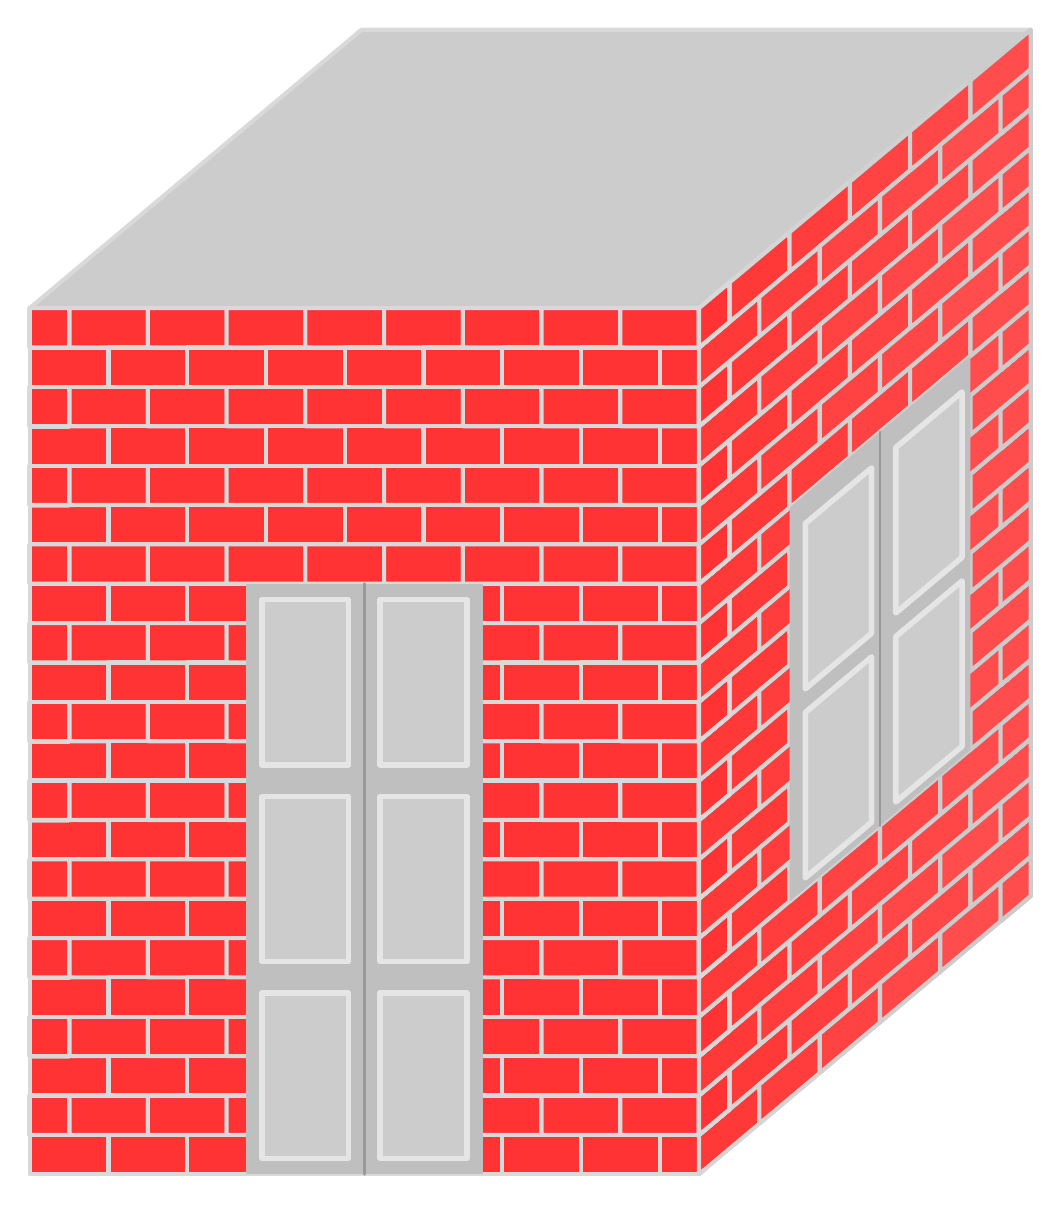
\begin{tikzpicture}[line join=round, line cap=round]
		\def\dg{1}%Độ dài viên gạch
		\def\goc{40}%Góc nghiêng nhìn mặt bên
		\def\n{8}%Số viên gạch một hàng mặt trước
		\def\m{5}%Số viên gạch một hàng mặt nghiêng
		\def\h{11}%1/2 Số hàng gạch (chiều cao)
		\colorlet{mgach}{red}%Màu viên gạch
		\colorlet{mvua}{gray}%Màu mạch vữa
		\pgfmathsetmacro{\rg}{\dg/2}%Chiều rộng viên gạch
		\pgfmathsetmacro{\ngang}{(2*\n+1)*\rg}
		\pgfmathsetmacro{\cao}{\h *\dg}
		\pgfmathsetmacro{\nghieng}{(2*\m+1)*\rg}
		%Mái:
		\draw[gray!30, fill=gray!40, line width=1.5] (0,\cao)--(\ngang,\cao)--([turn]\goc:\nghieng)--([turn]180-\goc:\ngang)--cycle;
		% Mặt trước
		\foreach \j in {1,...,\h}{
			\foreach \i in {1,...,\n}{
				\pgfmathsetmacro{\x}{(\i-1)*\dg}
				\pgfmathsetmacro{\y}{(\j-1)*2*\rg}
				\draw[mvua!30,fill=mgach!80, line width=1.5] (\x,\y)--(\x,\y+\rg)--([turn]-90:\dg)--([turn]-90:\rg)--cycle;
				\draw[mvua!30,fill=mgach!80, line width=1.5] (\n *\dg,\y)--(\n *\dg,\y+\rg)--([turn]-90:\rg)--([turn]-90:\rg)--cycle;
				\draw[mvua!30,fill=mgach!80, line width=1.5] (\x+\rg,\y+\rg)--(\x+\rg,\y+2*\rg)--([turn]-90:\dg)--([turn]-90:\rg)--cycle;
				\draw[mvua!30,fill=mgach!80, line width=1.5] (0,\y+\rg)--(0,\y+2*\rg)--([turn]-90:\rg)--([turn]-90:\rg)--cycle;
			}
		}
		%Mặt nghiêng
		\foreach \j in {1,...,\h}{
			\foreach \i in {1,...,\m}{
				\pgfmathsetmacro{\x}{\ngang+(\i-1)*\dg *cos(\goc)}
				\pgfmathsetmacro{\y}{(\i-1)*2*\rg *sin (\goc) +(\j-1)*2*\rg}
				\pgfmathsetmacro{\xc}{\ngang+(\m *\dg *cos(\goc))}
				\pgfmathsetmacro{\yc}{\m *2*\rg *sin (\goc) +(\j-1)*2*\rg}
				\pgfmathsetmacro{\xl}{\x+\rg *cos(\goc)}
				\pgfmathsetmacro{\yl}{\y+(1+sin(\goc)) *\rg}
				\pgfmathsetmacro{\xm}{\ngang}
				\pgfmathsetmacro{\ym}{2*(\j -1)*\rg+\rg}
				\pgfmathsetmacro{\hsmvua}{30+2*\i}
				\pgfmathsetmacro{\hsmgach}{80-2*\i}
				\draw[mvua!\hsmvua,fill=mgach!\hsmgach, line width=1.5] (\x,\y)--(\x,\y+\rg)--([turn]\goc-90:\dg)--([turn]-\goc-90:\rg)--cycle;
				\draw[mvua!\hsmvua,fill=mgach!\hsmgach, line width=1.5] (\xc,\yc)--(\xc,\yc+\rg)--([turn]\goc-90:\rg)--([turn]-\goc-90:\rg)--cycle;
				\draw[mvua!\hsmvua,fill=mgach!\hsmgach, line width=1.5] (\xl,\yl)--(\xl,\yl+\rg)--([turn]\goc-90:\dg)--([turn]-\goc-90:\rg)--cycle;
				\draw[mvua!30,fill=mgach!80, line width=1.5] (\xm,\ym)--(\xm,\ym+\rg)--([turn]\goc-90:\rg)--([turn]-\goc-90:\rg)--cycle;
			}
		}
		%Cửa trước
		\pgfmathsetmacro{\rc}{6*\rg}
		\pgfmathsetmacro{\cc}{15*\rg}
		\pgfmathsetmacro{\dc}{0.2}
		\pgfmathsetmacro{\xsh}{((2*\n +1)*\rg-\rc)/2}
		\fill[gray!50,shift={(\xsh,0)}](0,0)--(0,\cc)--([turn]-90:\rc)--([turn]-90:\cc)--cycle;
		\draw[gray!20,fill=gray!40,line width=2,shift={(\xsh+\dc,\dc)}] (0,0) --(0,\cc/3-2*\dc) --([turn]-90:\rc/2-2*\dc)--([turn]-90:\cc/3-2*\dc)--cycle;
		\draw[gray!20,fill=gray!40,line width=2,shift={(\xsh+\rc/2+\dc,\dc)}] (0,0) --(0,\cc/3-2*\dc) --([turn]-90:\rc/2-2*\dc)--([turn]-90:\cc/3-2*\dc)--cycle;
		\draw[gray!20,fill=gray!40,line width=2,shift={(\xsh+\dc,\cc/3+\dc)}] (0,0) --(0,\cc/3-2*\dc) --([turn]-90:\rc/2-2*\dc)--([turn]-90:\cc/3-2*\dc)--cycle;
		\draw[gray!20,fill=gray!40,line width=2,shift={(\xsh+\rc/2+\dc,\cc/3+\dc)}] (0,0) --(0,\cc/3-2*\dc) --([turn]-90:\rc/2-2*\dc)--([turn]-90:\cc/3-2*\dc)--cycle;
		\draw[gray!20,fill=gray!40,line width=2,shift={(\xsh+\dc,2*\cc/3+\dc)}] (0,0) --(0,\cc/3-2*\dc) --([turn]-90:\rc/2-2*\dc)--([turn]-90:\cc/3-2*\dc)--cycle;
		\draw[gray!20,fill=gray!40,line width=2,shift={(\xsh+\rc/2+\dc,2*\cc/3+\dc)}] (0,0) --(0,\cc/3-2*\dc) --([turn]-90:\rc/2-2*\dc)--([turn]-90:\cc/3-2*\dc)--cycle;
		\draw[gray!80,line width=1,shift={(\xsh+\rc/2,0)}](0,0)--(0,\cc);
		%cửa sổ
		\pgfmathsetmacro{\xshi}{(2*\n+1)*\rg+\rc *cos(\goc)/2}
		\pgfmathsetmacro{\yshi}{\cc/3+3*\rg *sin(\goc)}
		\pgfmathsetmacro{\xgcs}{\rc *cos(\goc)/2}
		\pgfmathsetmacro{\ygcs}{\rc *sin(\goc)/2}
		\fill[gray!50,shift={(\xshi,\yshi)}](0,0)--(0,2*\cc/3)--([turn]\goc-90:\rc)--([turn]-\goc-90:2*\cc/3)--cycle;
		\draw[gray!20,fill=gray!40,line width=2,shift={(\xshi+\dc,\yshi+1.5*\dc)}] (0,0) --(0,\cc/3-2*\dc) --([turn]\goc-90:\rc/2-2*\dc)--([turn]-\goc-90:\cc/3-2*\dc)--cycle;
		\draw[gray!20,fill=gray!40,line width=2,shift={(\xshi+\xgcs+\dc,\yshi+\ygcs+1.5*\dc)}] (0,0) --(0,\cc/3-2*\dc) --([turn]\goc-90:\rc/2-2*\dc)--([turn]-\goc-90:\cc/3-2*\dc)--cycle;
		\draw[gray!20,fill=gray!40,line width=2,shift={(\xshi+\dc,\cc/3+\yshi+\dc)}] (0,0) --(0,\cc/3-2*\dc) --([turn]\goc-90:\rc/2-2*\dc)--([turn]-\goc-90:\cc/3-2*\dc)--cycle;
		\draw[gray!20,fill=gray!40,line width=2,shift={(\xshi+\xgcs+\dc,\cc/3+\yshi +\ygcs+\dc)}] (0,0) --(0,\cc/3-2*\dc) --([turn]\goc-90:\rc/2-2*\dc)--([turn]-\goc-90:\cc/3-2*\dc)--cycle;
		\draw[gray!80,line width=1,shift={(\xshi+\xgcs,\yshi+\ygcs)}](0,0)--(0,2*\cc/3);
	\end{tikzpicture}
\end{document}